\section{Exploration de uintr}

\subsection{Prérequis est accès}

\begin{itemize}
  \item difficulté d'accès au processeur...
  \item J'ai eu accès au processeur ~2 mois 1/2 après le début du stage
  \item J'ai donc eu accès à une machine avec 2 CPU SPR... VPN... détails Saphir Rapid et VPN
  \item il faut une version patché du noyaux linux pour utilisé c'est nouvelle interruption
  Ce patch n'est pas disponible en mainline linux.
  J'ai donc télécharger le patch fourni par \intel{}, je l'ai compiler puis je l'ai installer sur la machine
  \item il faut compiler le noyau patché et activé les uintr dans le menu de configuration (il est aussi possible d'activé la posibilité que le kernel resoive l'interruption quand le processus est endormie en tache interruptible.)
  \item Pour utiliser les nouvelle instructions il faut une version récente de GCC... (version).
  Pas disponible avec LLVM-Clang
  \item pour compilé un programme il faut précié le flag de compilation \code{-muintr} pour les fichiers qui déclare un handler d'uintr.
\end{itemize}

\subsection{Fonctionnement des uintr}

\subsubsection{Les interruptions}

Pour commencer nous allons voire comment les interruption matérielle fonctionnent, elle sont nommé IRQ pour Interrupt ReQuest.
Nous allons utiliseront le terme interruption ordinaire ou IRQ.
Les interruption ordinaire existe depuis long temps est serve notamment à remonté des exceptions du processeur au noyau.
Nous allons nous concentrer sur l'envois d'interruption entre unité de calcule, donc entre processus.
Pour fonctionné les CPU on une unité dédié au traitement des interruption l'APIC pour Advanced Programmable Interrupt Controller.
Cette APIC permet au système de enregistré un handler pour chaque interruptions.
Pour ce faire le système une table \emph{IDT} (Interrupt Descriptor Table) qui contiens 256 entrées.
Donc 256 interruptions possible, les valeurs entre 0 et 255 sont aussi appelé vecteur.
Les vecteur compris entre 0 et 31 sont réservé pour les exceptions et interruption système, ce entre 32 et 127 sont réservé pour les interruptions pour les périphériques,
128 est réservé pour les appel système et entre 129 et 255 pour des utilisation varier.

Il est important de savoir que chaque unité de calcul (coeur logique) possède un \emph{APIC ID} physique.
Petit fun-fact le \emph{core ID} est un sous ensemble de l'\emph{APIC ID}.

Pour déclencher une interruption il y a quatre possibilités :

\begin{enumerate}
  \item Une exceptions déclencher par le CPU (e.g. division par zero, défaut de segmentation...).
  \item Une instruction comme \code{INT80 numSysCall} pour déclencher un appel système ou bien \code{INT3} pour définir un point d'arrêt, ou encore \code{INTO}, \code{BOUND} et \code{INT n}.
  \item Des pins du processeur dédier à la réception d'interruption lancer à partir d'un périphérique.
  \item Demander à l'APIC en lui même grâce à un registre ICR pour Interrupt Command Register.
  Il existe un ICR par vecteur il faut donc écrire l'\emph{APIC ID} du destinataire dans le ICR du vecteur que l'on veut déclencher.
  Seul le CPU et le noyau peuvent modifier les ICR.
\end{enumerate}

On vois bien que les IRQ fonction au niveau du noyau et du CPU.

Nous allons voir un example d'envoi d'IRQ entre 2 processus en cours d'execution.
Tous d'abort l'initialisation ce fait au démarrage du système et consiste principalement à définir les handler noyau dans l'\emph{IDT}.
Au préalable il faut définir le vecteur utiliser, le handler noyau, la technique pour contacté le système et l'identification du récepteur (e.g. par un patch du noyau, par un module noyau...).

Nous allons maintenant voir les états de l'envois d'une IRQ montré sur la figure suivant \ref{fig:sendInt}.

\begin{enumerate}[label=\protect\circled{\arabic*}]
  \item Le récepteur fait un appel système pour indique au noyau comment il veut être avertie d'une interruption (e.g. un handler utilisateur, un descripteur de fichiers qu'il vas lire, un appel système bloquante, une zone mémoire ou écrire...).
  \item l'émetteur peut donc avertir le noyau qu'il fau envoyer une interruption pour cela il peut utiliser un appel système ou écrire dans un descripteur de fichiers...
  \item Le noyau détermine l'unité de calcule ou ce trouve le récepteur. Pour cela il peut utiliser par example un \emph{PID} (Processus ID) donné par l'émetteur ou autre.
  Il vas donc pouvoir détermine le \emph{APIC ID} de unité de calcul à interrompre.
  \item Le noyau écrire donc l'\emph{APIC ID} dans le \emph{ICR} d'un vecteur détermine à l'avance. L'émetteur vas reprendre la main après un autre changement de contexte.
  \item L'APIC vas donc interrompre le récepteur qui vas donc stoppé sont execution est passer dans le noyau.
  Une fois dans le noyau le handler vas ce déclencher et exécuté le code prévue au préalable (déclenchement d'un handler utilisateur, écrire dans un descripteur de fichiers, écrire dans une zone mémoire...).
\end{enumerate}

\begin{figure}[H]
  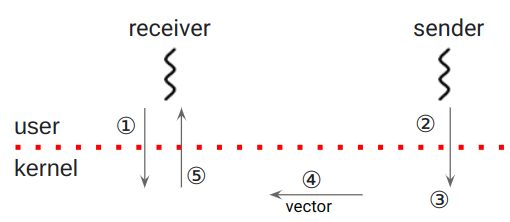
\includegraphics[width=\textwidth]{images/interruptSend.png}
  \caption{L'envois d'une interruption}
  \label{fig:sendInt}
\end{figure}

Il est possible de masquer les interruptions grâce à deux instructions utilisable seulement par le noyau qui sont \code{clui} et \code{stui}.
Ces interruption modifie un flag (\emph{IF}) qui ce trouve dans le registre d'états de l'unité de calcul \code{RFLAGS} (aussi nommé \code{EFLAGS} sur les architecture 32bits).
La liste des interruptions pour les IRQ ce trouve ici\ref{interruptInstructions}.

Comment on la vue ce mécanisme fonction totalement dans le noyau du système.
Dans notre example il faut au minimum deux changement de contexte (context switch) pour le récepteur et l'émetteur et même peut être plus si le récepteur dois déclenché un handler coté utilisateur.

% Il fau noté que les registre 32 bit commance par un E et les 64 bit par un R (ex: EIP et RIP).
% RIP is Register Instructions Pointer, RFLAGS is Register with all core FLAGS (OF, CF, IF...), RSP is Register Stack Pointer, CS is Code Section, IF is Interrupt Flag store in EFLAGS

\subsubsection{Détail}

TODO: ...

Le mécanisme est composé de 5 instruction que l'on peut retrouvé dans le table TODO: ref.

\begin{itemize}
  \item 5 instructions
  \item registre MSR pour l'init
\end{itemize}

\begin{figure}[H]
  \begin{tabular}{|l|l| }
    \hline
    \bf Interruption & \bf Interruption en espace utilisateur\\
    \hline
    cli (CLear Interrupt flag) & clui (CLear User Interrupt flag)\\
    \hline
    sti (SeT Interrupt flag) & stui (SeT User Interrupt flag)\\
    \hline
    & testui (Read User Interrupt flag)\\
    \hline
    iret (Interrupt RETurn) & uiret (User Interrupt RETurn)\\
    \hline
    \multirow{3}{0.5\textwidth}{APIC pin, APIC ICR \code{INT n}, \code{INT3}, \code{INTO}, \code{BOUND}, \code{INT80 n} et registre IRQ} & sendipi <uipi_index>\\
    &\\
    &\\
    &\\
    \hline
    % \multicolumn{2}{|c|}{...} \\
    % \hline
  \end{tabular}
  \caption{Instructions des interruption et interruption en espace utilisateur}
  \label{interruptInstructions}
\end{figure}


% interrupt invoked (push oldRSP, RFLAGS, CS, RIP, errorCode (IRQ vector value ?))
% IRET (pop errorCode, RIP, CS, RFLAGS, oldRSP)
% uintr invoked (push oldRSP, RFLAGS, RIP, UIRRV)
% uiret (pop UIRRV, RIP, RFLAGS, oldRSP)

\subsubsection{Capacité présente et futur}

\begin{itemize}
  \item process => process
  \item kernel => process
  \item device => process
  \item au niveaux des thread...
  \item chaque thread peut avoir un seul thread de défini.
  \item Il existe 64 vecteur entre 0 et 63
  \item masquage
  \item le thread dois être en ring-3
  \item peut fonctionné si le thread est endormi mais j'ai pas testé car ...
  \item l'interruption est délivré si le processus est en mode utilisateur. Le comportement par defaut et que l'interruption est reçus quand le thread est à nouveau au espace utilisateur.
  \item Si on à configuré dans à la compilation du noyau il est possible de donné 3 flags au moment de lenregistrement du handler. Le premier flag UINTR_HANDLER_FLAG_WAITING_ANY pour activé le fait de pouvoir recesoire une interruption quand le processus n'est pas ordonacé ou est dans un appel système interruptible. Les 2 flague suivant UINTR_HANDLER_FLAG_WAITING_RECEIVER, UINTR_HANDLER_FLAG_WAITING_SENDER s'ajoute au flague préciédent et précide si le cout du context switch est pour l'émetteur ou le recepteur de l'interruption.
  \item Le fonctionnement à partir du kernel est très similaire au fonctionnemt des inrettruption "ordinaire" plus l'appel du handler en espace utilisateur.
\end{itemize}

\subsubsection{Example}

\begin{itemize}
  \item example avec schéma
\end{itemize}

\begin{figure}[H]
  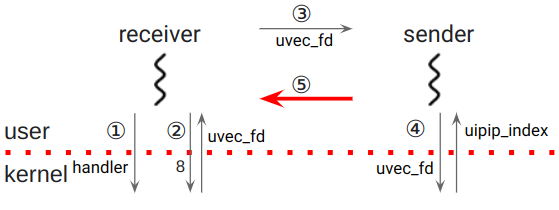
\includegraphics[width=\textwidth]{images/uintrInit.png}
  \caption{Phase d'initialisation des uintr}
  \label{fig:initUintr}
\end{figure}
\begin{figure}[H]
  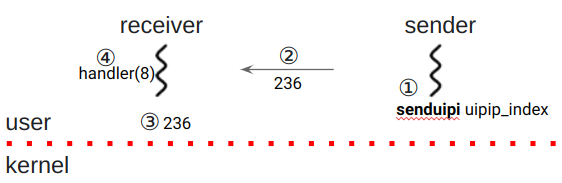
\includegraphics[width=\textwidth]{images/uintrSend.png}
  \caption{L'envois d'une uintr}
  \label{fig:sendUintr}
\end{figure}

\subsubsection{Partage du FD}

\begin{itemize}
  \item Pour mes testes "jouer" j'ai utiliser \verb|uintr_register_self()|
  \item pipe / socket / URL pour NewMadeleine (on en reparle en section XXX)
  \item inheritance / pidfd_getfd / sockets
  \item \verb|pidfd_getfd|
\end{itemize}

\subsubsection{+}

\begin{itemize}
  \item comparé au signaux ?
  \item TODO ...
  \item faire attetion tous les registre ne sont pas sauvegardé. La responsabilité de la sauvegarde est à l'utilisateur. Pour ça le compilateur permet de sauvegardé les registre généraux mais pas les vecteur SIMD. Donc il faut évité de les utilisé ou les sauvegardé avant.
  \item On ne peut pas attendre dans un handler donc on peut appelé seulement les focntion et appel système async safe, on en reparlera dans le chapitre TODO: cite. En plus il faut faire attention au operations sur les chaine de caractére de la libc memcpy, memmove, memset et memcmp qui utiliser des registre, il est possible de les inline sans utiliser de vecteur SIMD grâce au flag de compilation \code{-minline-all-stringops}.
\end{itemize}

\subsection{Tests du mécanisme}

% sur un exemple minimal en communication inter-processus

\begin{itemize}
  \item entre process
  \item entre threads
  \item avec alt stack
  \item test d'écrasement des interruptions
  \item avec binding (plus pourquoi avec binding que comparaison avec et sans)
  \item avec turbo boost
\end{itemize}

\subsection{Correction du patch pour l'appel système uintr_alt_stack}

TODO

\subsection{Mesure de la latence (Feedback Mathieu)}

TODO: expliquer que le binding est important

\subsection{Performances}

TODO

\begin{itemize}
  \item Dans un premier temps j'ai pas bind les thread par pu donc j'avais de mauvais résultats.
  \item J'ai fait différents bind (on vois que c'est similaire sauf quand on passe entre 2 NUMA)
  \item si on monte la frequence c'est mieux (turbo boost)
  \item 
\end{itemize}
